\section{User Interface}
Considering the application is only a \acrshort{poc} there is almost no focus on the \acrlong{poc} nor on the \acrfull{ux}. To at least give a slight indication of what information needs to be displayed where, a \acrshort{ui} mock-up is created in Adobe Xd, Adobe Xd is a lightweight, rudimentary visual editor that enables designers to quickly develop and share interactive prototypes. A few example screens of the \acrshort{ui} prototype can be found below.
\begin{figure}[H]
\centering
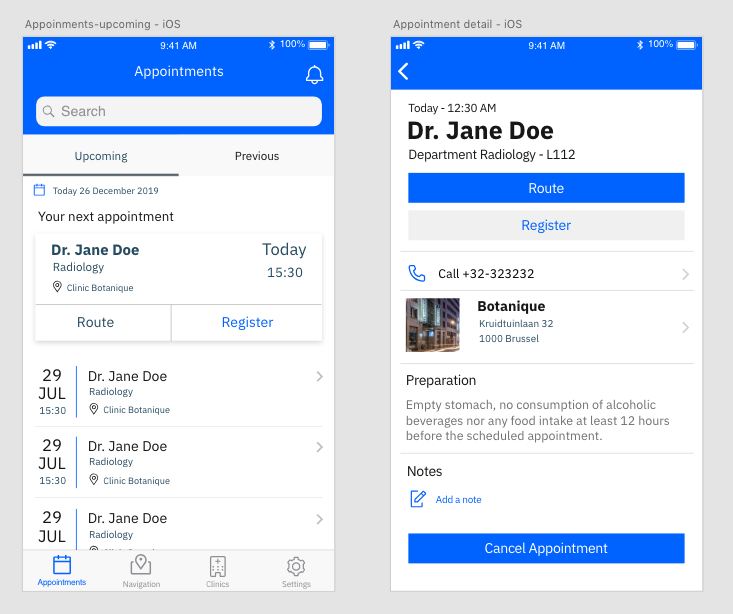
\includegraphics[scale=0.5]{appointments_screen_ios}
\caption{User interface of the appointments and detailed view for iOS}
\end{figure}
\begin{figure}[H]
\centering
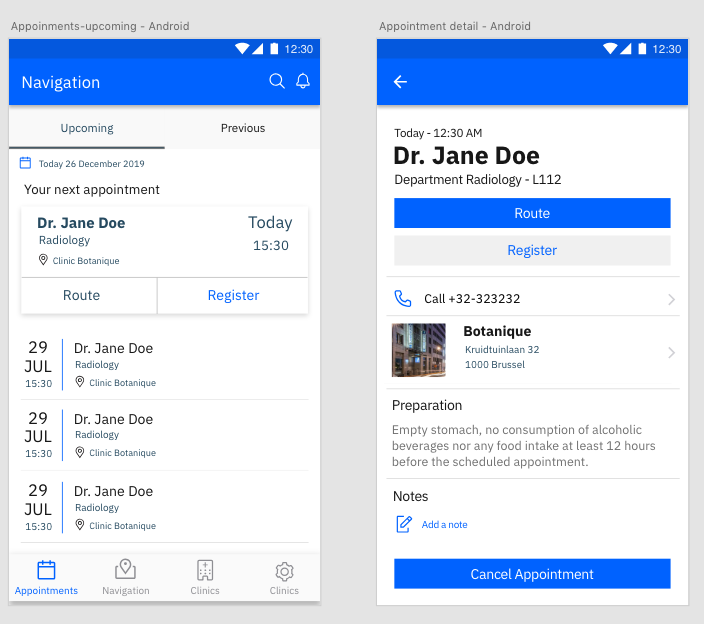
\includegraphics[scale=0.5]{appointments_screen_android}
\caption{User interface of the appointments and detailed view for Android}
\end{figure}
\begin{figure}[H]
\centering
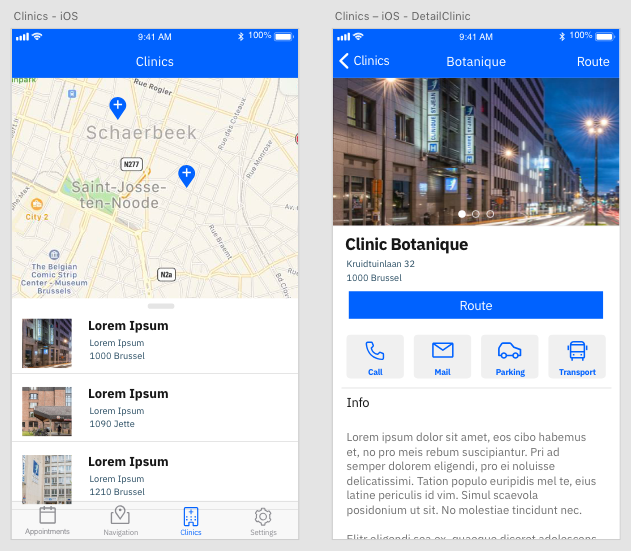
\includegraphics[scale=0.5]{clinics_screen_ios}
\caption{User interface of the hospital venues and detailed view for iOS}
\end{figure}
\begin{figure}[H]
\centering
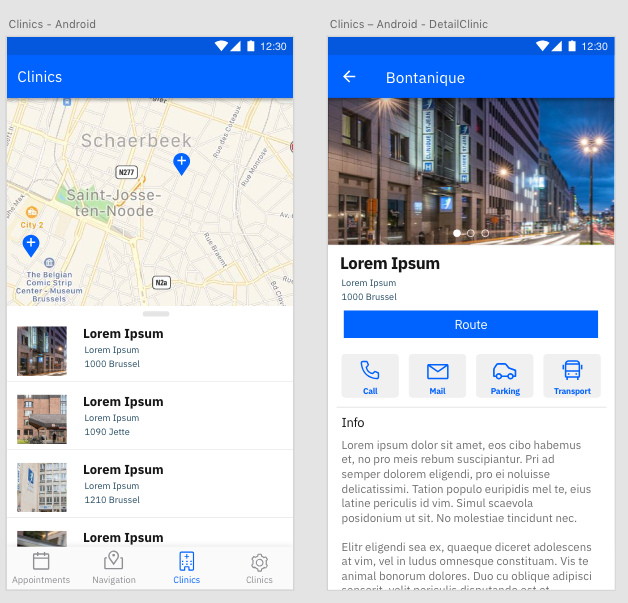
\includegraphics[scale=0.5]{clinics_screen_android}
\caption{User interface of the hospital venues and detailed view for Android}
\end{figure}
\section{Database Communication}
\subsection{Implementing Repository Pattern}
In practice, implementing the repository pattern in Android comes with some difficulties. Firstly dependency injection needs to be handled in a modular fashion, to attain the testable individual modules, the handling of dependency injection is covered in the next topic. Secondly, one must provide two types of data communications: online and offline. 
\section{Dependency Injection using Dagger2}
To remove the abstraction of the different methods of dependency injection, the library Dagger2 (supported by Google) is used. This library sets up the required dependencies throughout the application and registers them accordingly. Upon launching a class that requires a dependency, the Dagger2 instance will load them as specified in the AppModule. Since the architecture used in the application is \acrshort{mvvm}, the ViewModel is injected into an activity. The following code contains an AppModule, AppComponent, ViewModelFactoryModule and a subclass of the Application class, used for casting an activity:
\begin{verbatim}
/**
 * Component to be used to handle dependency injection
 */
@Singleton
@Component(modules = [AppModule::class, ViewModelModule::class])
interface AppComponent {
    fun inject(target: AppointmentList)
}

/**
 * Module that can be used to declare dependencies
 */
@Module
class AppModule @Inject constructor(private val app: Application) {
    @Provides
    @Singleton
    fun providesApplication(): Application {
        return app
    }

    @Provides
    @Singleton
    fun providesAppointmentViewModel(app: Application):
    AppointmentViewModel {
        return AppointmentViewModel(app, providesWebService())
    }

    @Singleton
    @Provides
    fun providesWebService(): WebService {
        return Retrofit.Builder()
            .baseUrl(Constants.BASE_URL)
            .addConverterFactory(GsonConverterFactory.create())
            .build()
            .create(WebService::class.java)
    }

    @Provides
    @Singleton
    fun providesAppointmentDao(db: AppDataBase): AppointmentDao {
        return db.appointmentDao()
    }

    @Provides
    @Singleton
    fun providesAppDatabase(app: Application): AppDataBase {
        return Room.databaseBuilder(
            app,
            AppDataBase::class.java, "app_database"
        ).fallbackToDestructiveMigration().allowMainThreadQueries().build()
    }
}


/**
 * Child Application Class to use for casting inside an activity
 * Create the AppComponent reference and uses this 
 * for injecting inside an Activity
 */
class DependencyApplication : Application() {
    lateinit var appComponent: AppComponent

    override fun onCreate() {
        super.onCreate()
        appComponent = initDagger(this)
    }

    private fun initDagger(app: DependencyApplication): AppComponent = 
    DaggerAppComponent.builder().appModule(AppModule(app)).build()

}

**
 * Factory to get the ViewModel by class for DI
 */
@Singleton
class DaggerViewModelFactory @Inject constructor(
    private val creators: Map<Class<out ViewModel>,
    @JvmSuppressWildcards Provider<ViewModel>>
) : ViewModelProvider.Factory {

    @Suppress("UNCHECKED_CAST")
    override fun <T : ViewModel> create(modelClass: Class<T>): T {
        var creator: Provider<out ViewModel>? = creators[modelClass]
        if (creator == null) {
            for ((key, value) in creators) {
                if (modelClass.isAssignableFrom(key)) {
                    creator = value
                    break
                }
            }
        }
        if (creator == null) {
            throw IllegalArgumentException("unknown model class $modelClass")
        }
        try {
            return creator.get() as T
        } catch (e: Exception) {
            throw RuntimeException(e)
        }
    }
}

@MustBeDocumented
@Target(AnnotationTarget.FUNCTION)
@Retention(AnnotationRetention.RUNTIME)
@MapKey
annotation class ViewModelKey(val value: KClass<out ViewModel>)

/**
 * Module to inject ViewModel instances
 */
@Module
abstract class ViewModelModule {

    @Binds
    abstract fun bindViewModelFactory(factory: DaggerViewModelFactory): 
    ViewModelProvider.Factory

    @Binds
    @IntoMap
    @ViewModelKey(AppointmentViewModel::class)
    abstract fun bindAppointmentsListActivity(vm: AppointmentViewModel): 
    ViewModel
}
\end{verbatim}
The injection of the dependency into the AppointmentList fragment is done using the following code:

\begin{verbatim}
class AppointmentList : Fragment() {
    @Inject
    lateinit var viewModelFactory: ViewModelProvider.Factory

    override fun onCreateView(
        inflater: LayoutInflater, container: ViewGroup?,
        savedInstanceState: Bundle?
    ): View? {
        val view = inflater.inflate(R.layout.fragment_appointment_list, container, false)
        (this.activity!!.application as DependencyApplication).appComponent.inject(this@AppointmentList )
        val appointmentViewModel = ViewModelProviders.of(this, viewModelFactory)[AppointmentViewModel::class.java]

        //Recyclerview
        val viewManager = LinearLayoutManager(this.context)
        val viewAdapter = AppointmentsAdapter()

        val recyclerview = view.findViewById<RecyclerView>(com.ibm.geolocationframework.R.id.rv_appointments).apply {
            setHasFixedSize(true)
            layoutManager = viewManager
            adapter = viewAdapter
        }
        appointmentViewModel.getAppointments().observe(this, Observer<List<Appointment>> { appointmentList ->
            viewAdapter.setAppointments(appointmentList)
        })
        // Inflate the layout for this fragment
        return view
    }

    companion object {
        @JvmStatic
        fun newInstance() =
            AppointmentList().apply {}
    }
}
\end{verbatim}
\subsection{Testing API}
To aid in testing the database a test \acrshort{api} is programmed using a Node.js framework: Express. it is a very simple tool to create a web \acrshort{api} ready for consumption \cite{Express2019}. The testing \acrshort{api} is structured according to the entities specified in the \acrshort{uml} diagram with the corresponding relations. For this specific application there are a couple of endpoints exposed for requests:
\begin{itemize}
\item GET /appointments - this returns a JSON array containing test appointments;
\item GET /hospital - this returns information about the hospital such as address, contact details and venues;
\item GET /doctors - this fetches all the doctors present in the hospital records;
\item GET /departments - this returns all the departments available in the hospital and its venues;
\end{itemize}
\subsubsection{Faker}
Instead of using ad random numerical combinations or lorem ipsum texts, a library called Faker is used to generate different random values such are names, addresses, e-mail addresses and phone numbers. Faker is available for almost every general purpose language and is easy to use. It is always easier to work with representative data than it is to work with 'lorem ipsum' or '123456789' \cite{DanieleFaraglia2014}.
\subsection{IBM BlueMix API}
The existing \acrshort{api} developed by IBM provides the application with a list of appointments (testing mode). An example of the JSON output can be found below:

\begin{verbatim}
[
    {
        "appointmentId": "000010130000001",
        "appointmentTime": "2017-10-16T14:14:00+02:00",
        "patientNr": 2000000420,
        "patientName": "SMITH, JULIE",
        "doctorNr": 123456,
        "doctorName": "FELDUNS, JEAN",
        "departmentId": "I",
        "departmentName": "USI",
        "siteId": "BO",
        "siteName": "Botanique",
        "appointmentReason": "Consultation Orthopédique",
        "appointmentInstruction": "La pendule fait",
        "appointmentStatus": "E",
        "appointmentStatusDescription": "Evaluated"
    }
]
\end{verbatim}			
\subsubsection{Entities}
The specific entities used throughout this application are:
\begin{itemize}
\item appointment;
\item hospital;
\item sites - the different locations of a hospital;
\item doctor;
\item patient;
\item department;
\end{itemize}
\section{Testing Application Programming Interface}
\section{Tools and frameworks used}
\section{MapWize}
MapWize is a service that digitalizes architectural plans and makes them interactive. MapWize offers an online environment in which you can easily create floor plans that can be used by the \acrshort{sdk}. In the online editor you can declare specific points of interest (PoIs) and routes from and to points. The creation of a digital map for testing purposes is out of scope for this thesis.
\subsection{MapWize SDK}
The team of developers at MapWize developed a completely open source \acrshort{sdk}, targeting the following platforms: iOS, Android, JS and \acrfull{pwa} \cite{MapWize.io2019a}. The one for Android has three versions: ready to use UI, bare-bones and an embedded WebView component.
\subsubsection{MapWize Barebone versus MapWize UI}
The bare-bones version of the \acrshort{sdk} comes as a plugin on top of the MapBox OpenGL library for Android. The Mapbox library handles the embedding of interactive vector assets into mobile applications \cite{Mabox2019}, this library is out of scope for this thesis, it is sufficient to know its function inside the MapWize \acrshort{sdk}. 

\section{Cisco Connectected Mobile Experiences integration}
The manner in which the position of a patient is retrieved is based on the nearest WiFi router of Cisco.
\subsection{Function of Cisco CMX}

\section{IndoorLocation Framework}
The IndoorLocation framework is one heavily used in conjunction with MapWize, it is a framework that allows developer to use geolocalization based on numerous indoor positioning technologies (IPS) such are: GPS, beacons, Wi-Fi, Li-Fi, Ultrasounds etc \cite{IndoorLocation.io2019}.

\section{Theoretical Features}
\subsection{Mobility Indicator}
\subsection{Safety Cultivation}
\subsection{Efficient Path Mapping}


